
\fullcite{vosc15}

This is a nice and technical article with a thorough description of the 
FEM discretisation. Added bonus, in 3d. 

\begin{multicols}{2}
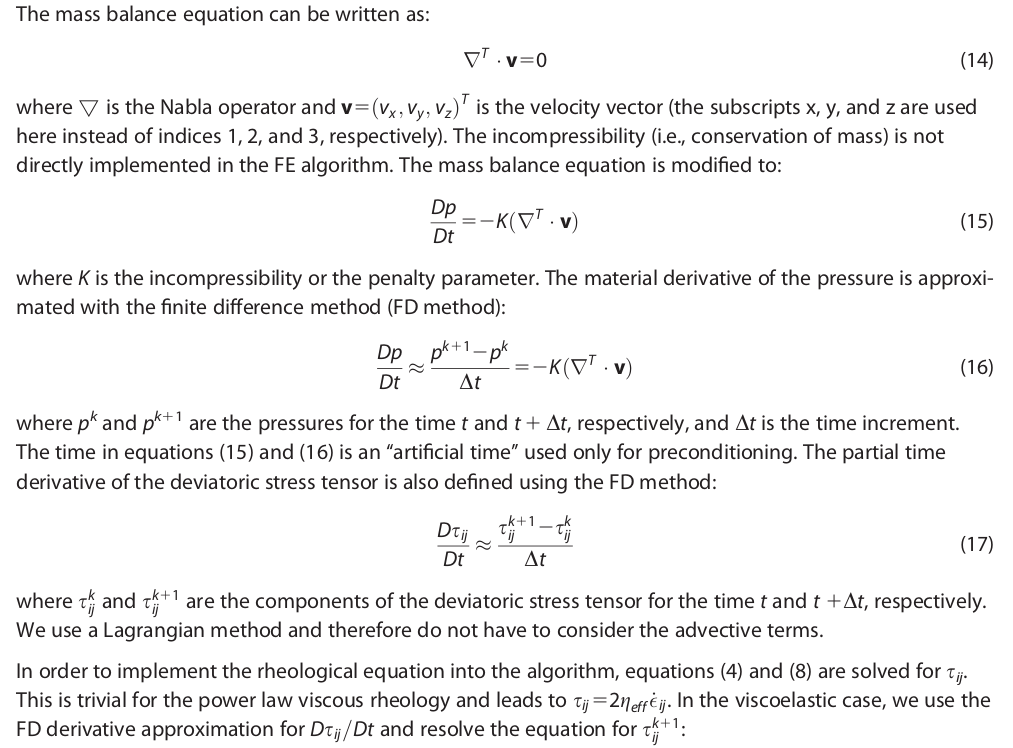
\includegraphics[width=8.25cm]{images/viscoelasticity/vosc15_l}\\
\[
\frac{Dp}{Dt} = -K \vec\nabla\cdot \vec\upnu
\]
\[
\frac{Dp}{Dt} \simeq \frac{p^{k+1} -p^k}{\delta t} = -K \vec\nabla\cdot \vec\upnu
\]
\end{multicols}

\begin{multicols}{2}
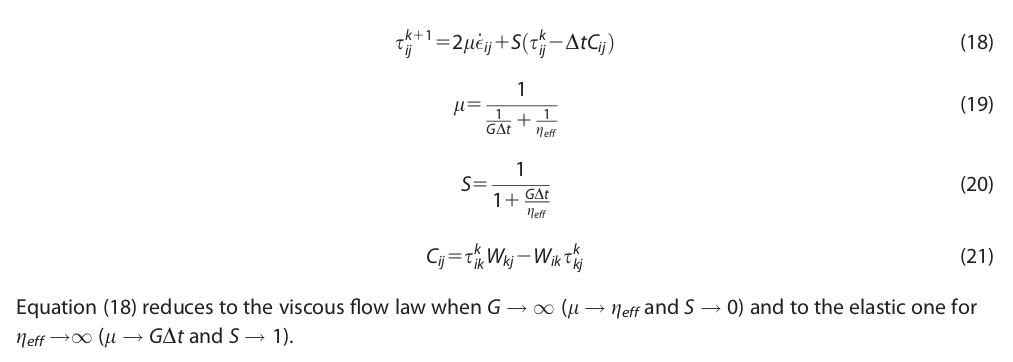
\includegraphics[width=8.25cm]{images/viscoelasticity/vosc15_m}\\
\[
\tau_{ij}^{k+1} = 2 \eta_{ve} \dot{\varepsilon}_{ij} + \left(1+\frac{G \delta t}{\eta}\right)^{-1} 
( \tau_{ij}^k - \tau^k_{ik} \omega_{kj} - \omega_{ik} \tau{kj}^k)
\]
with
\[
\eta_{ve}= \left(  \frac{1}{\eta} + \frac{1}{G \delta t} \right)^{-1}
\]

{\color{red} how to name S? }

\end{multicols}


\begin{multicols}{2}

\includegraphics[width=8.25cm]{images/viscoelasticity/vosc15_a}\\
\[
\vec\nabla \cdot \vec\upnu = 0
\]
\end{multicols}

\begin{multicols}{2}
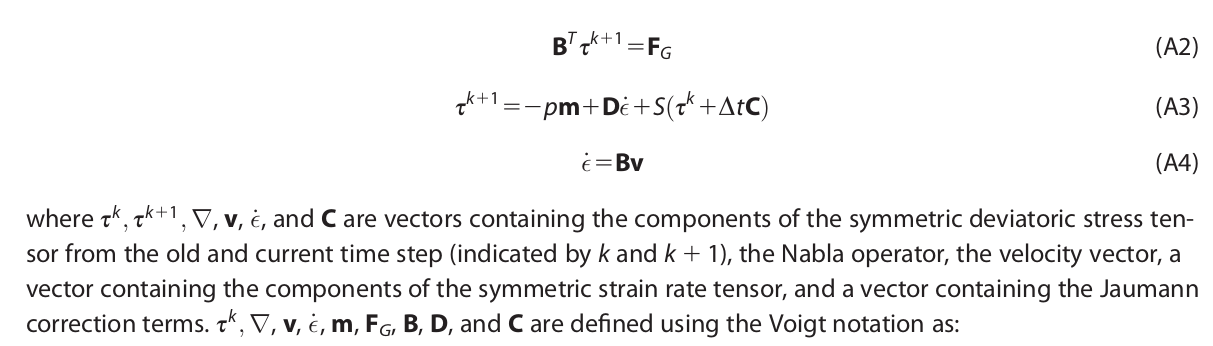
\includegraphics[width=8.25cm]{images/viscoelasticity/vosc15_b}\\
\[
\vec\tau^{k+1} = -p \vec{m}  + {\bm D} \cdot \vec{\varepsilon} 
+ S (\vec\tau^k + \delta t \; \vec{C})
\]
\end{multicols}

\begin{multicols}{2}
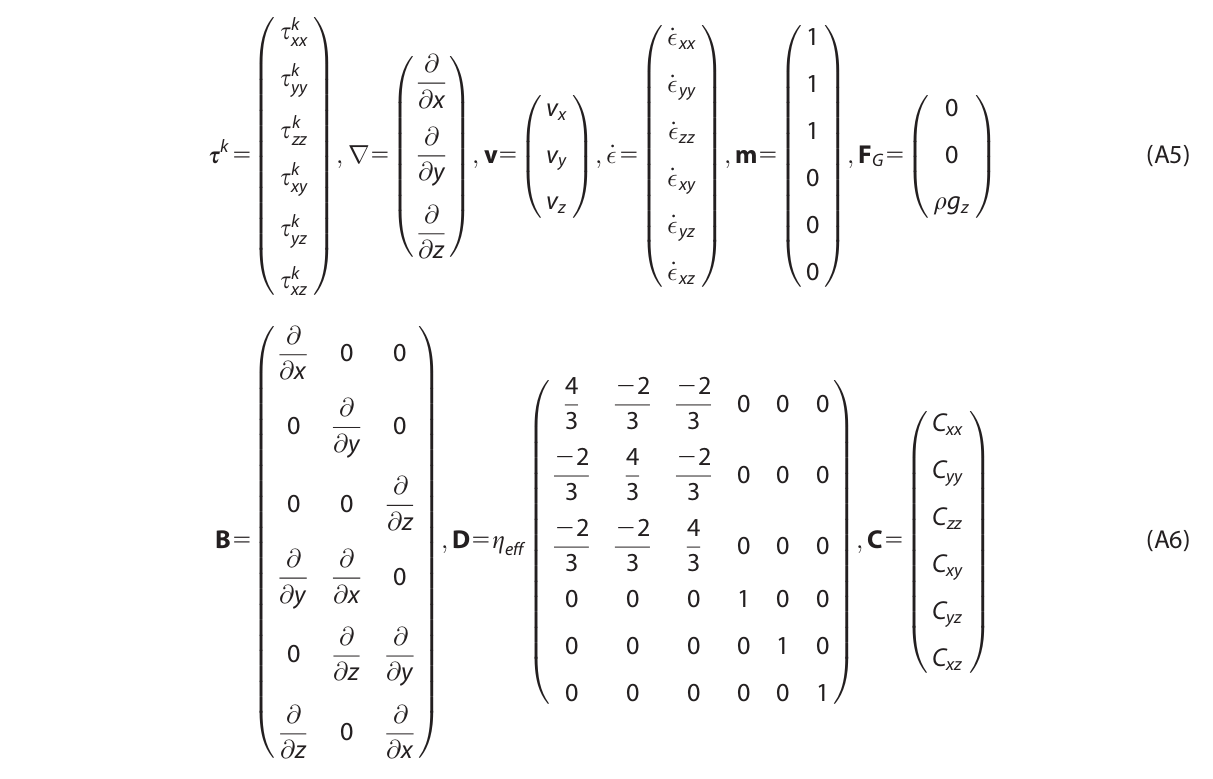
\includegraphics[width=8.25cm]{images/viscoelasticity/vosc15_c}
\end{multicols}

\begin{multicols}{2}
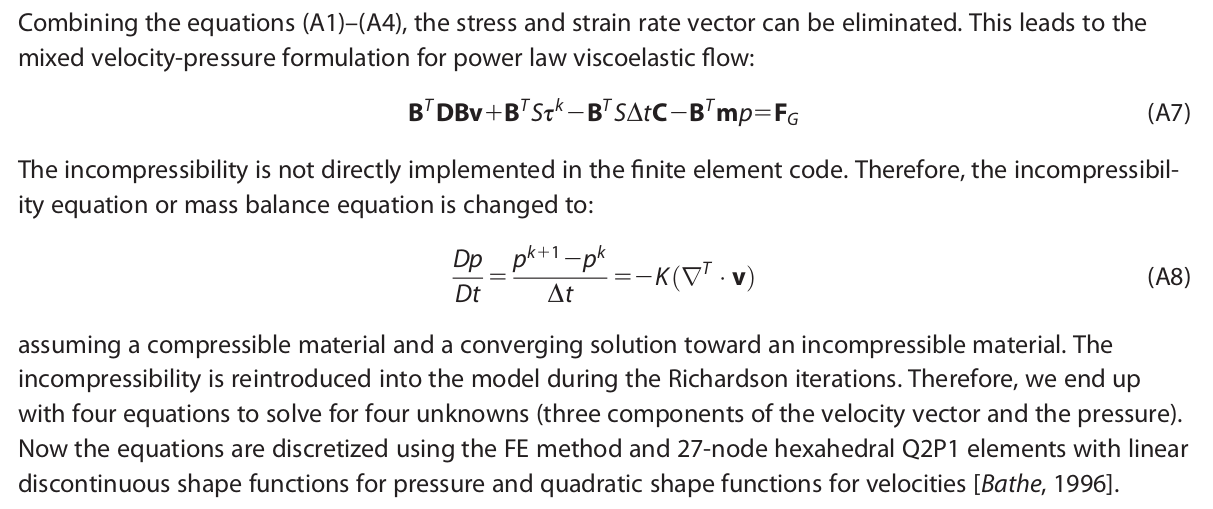
\includegraphics[width=8.25cm]{images/viscoelasticity/vosc15_d}
\end{multicols}


\begin{multicols}{2}
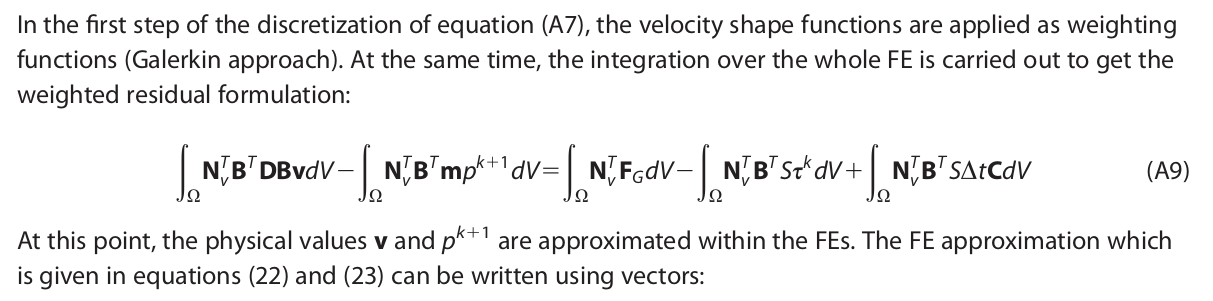
\includegraphics[width=8.25cm]{images/viscoelasticity/vosc15_e}
\end{multicols}

\begin{multicols}{2}
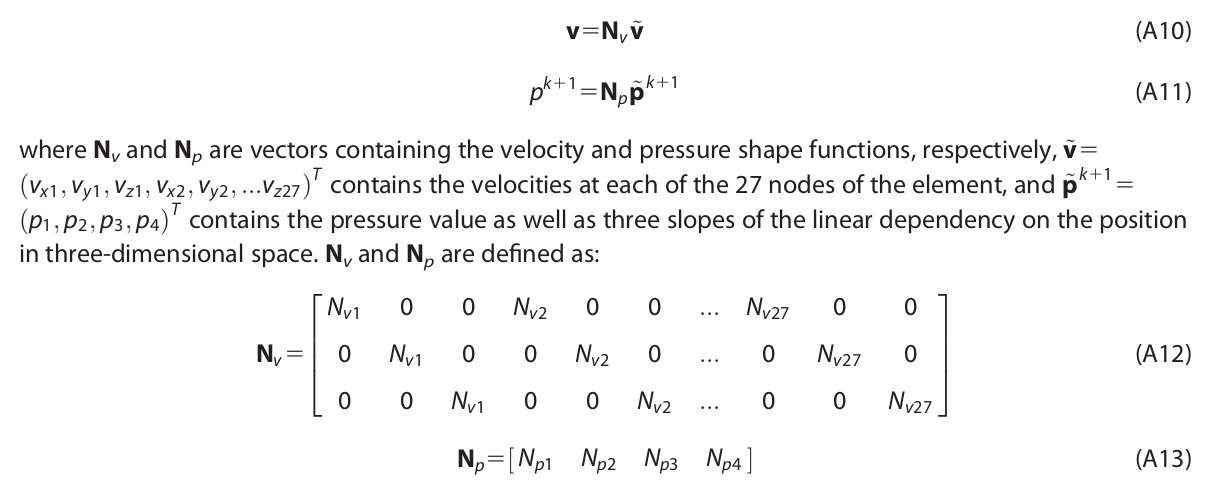
\includegraphics[width=8.25cm]{images/viscoelasticity/vosc15_f}
\end{multicols}

\begin{multicols}{2}
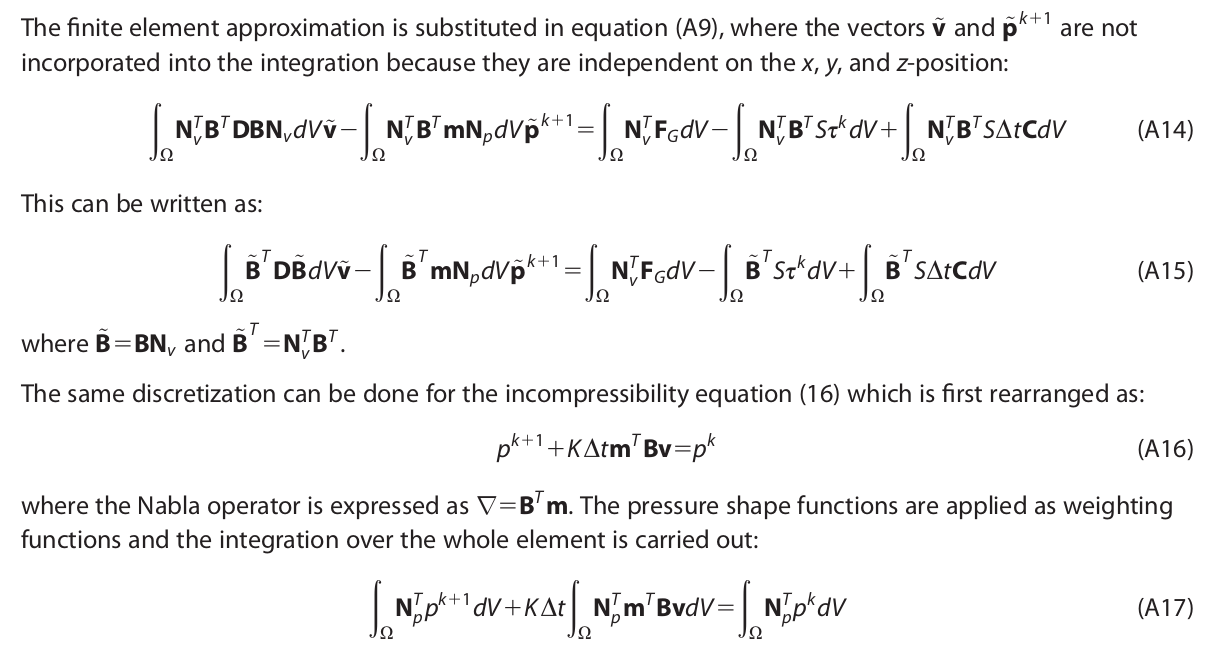
\includegraphics[width=8.25cm]{images/viscoelasticity/vosc15_g}
\end{multicols}

\begin{multicols}{2}
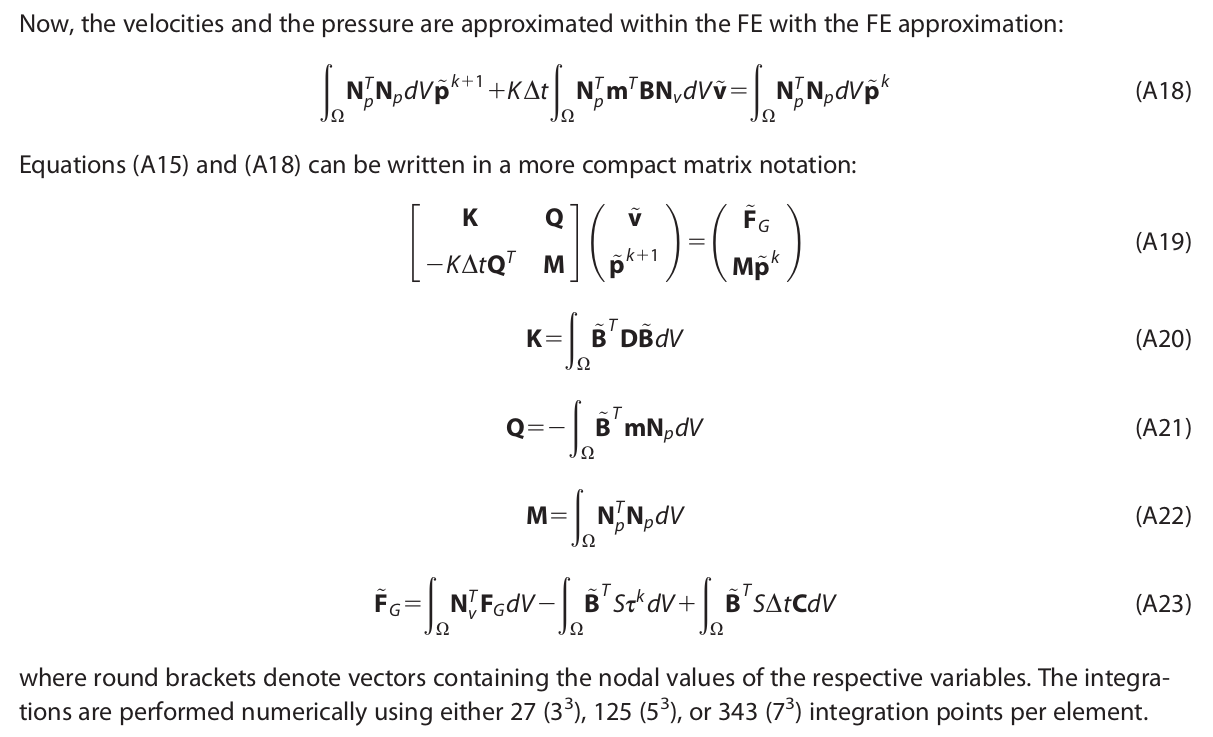
\includegraphics[width=8.25cm]{images/viscoelasticity/vosc15_h}
\end{multicols}

\begin{multicols}{2}
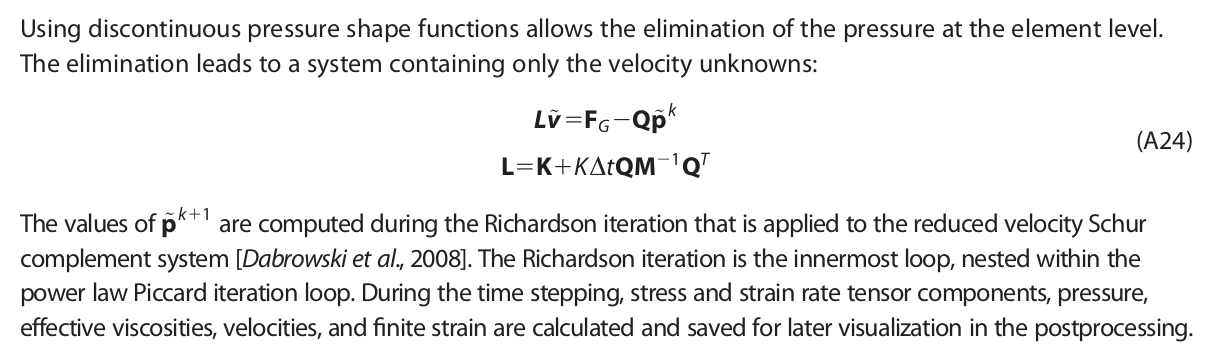
\includegraphics[width=8.25cm]{images/viscoelasticity/vosc15_i}
\end{multicols}






